\documentclass[]{article}
\usepackage{lmodern}
\usepackage{amssymb,amsmath}
\usepackage{ifxetex,ifluatex}
\usepackage{fixltx2e} % provides \textsubscript
\ifnum 0\ifxetex 1\fi\ifluatex 1\fi=0 % if pdftex
  \usepackage[T1]{fontenc}
  \usepackage[utf8]{inputenc}
\else % if luatex or xelatex
  \ifxetex
    \usepackage{mathspec}
  \else
    \usepackage{fontspec}
  \fi
  \defaultfontfeatures{Ligatures=TeX,Scale=MatchLowercase}
\fi
% use upquote if available, for straight quotes in verbatim environments
\IfFileExists{upquote.sty}{\usepackage{upquote}}{}
% use microtype if available
\IfFileExists{microtype.sty}{%
\usepackage{microtype}
\UseMicrotypeSet[protrusion]{basicmath} % disable protrusion for tt fonts
}{}
\usepackage[margin=1in]{geometry}
\usepackage{hyperref}
\hypersetup{unicode=true,
            pdftitle={Causal Inference Final Project: Effect of Smoking on 10-year Development of Coronary Heart Disease},
            pdfauthor={Bianca Doone, Michael Attah, Graham Casey Gibson, Daniel Saunders, Nutcha Wattanachit},
            pdfborder={0 0 0},
            breaklinks=true}
\urlstyle{same}  % don't use monospace font for urls
\usepackage{color}
\usepackage{fancyvrb}
\newcommand{\VerbBar}{|}
\newcommand{\VERB}{\Verb[commandchars=\\\{\}]}
\DefineVerbatimEnvironment{Highlighting}{Verbatim}{commandchars=\\\{\}}
% Add ',fontsize=\small' for more characters per line
\usepackage{framed}
\definecolor{shadecolor}{RGB}{248,248,248}
\newenvironment{Shaded}{\begin{snugshade}}{\end{snugshade}}
\newcommand{\KeywordTok}[1]{\textcolor[rgb]{0.13,0.29,0.53}{\textbf{#1}}}
\newcommand{\DataTypeTok}[1]{\textcolor[rgb]{0.13,0.29,0.53}{#1}}
\newcommand{\DecValTok}[1]{\textcolor[rgb]{0.00,0.00,0.81}{#1}}
\newcommand{\BaseNTok}[1]{\textcolor[rgb]{0.00,0.00,0.81}{#1}}
\newcommand{\FloatTok}[1]{\textcolor[rgb]{0.00,0.00,0.81}{#1}}
\newcommand{\ConstantTok}[1]{\textcolor[rgb]{0.00,0.00,0.00}{#1}}
\newcommand{\CharTok}[1]{\textcolor[rgb]{0.31,0.60,0.02}{#1}}
\newcommand{\SpecialCharTok}[1]{\textcolor[rgb]{0.00,0.00,0.00}{#1}}
\newcommand{\StringTok}[1]{\textcolor[rgb]{0.31,0.60,0.02}{#1}}
\newcommand{\VerbatimStringTok}[1]{\textcolor[rgb]{0.31,0.60,0.02}{#1}}
\newcommand{\SpecialStringTok}[1]{\textcolor[rgb]{0.31,0.60,0.02}{#1}}
\newcommand{\ImportTok}[1]{#1}
\newcommand{\CommentTok}[1]{\textcolor[rgb]{0.56,0.35,0.01}{\textit{#1}}}
\newcommand{\DocumentationTok}[1]{\textcolor[rgb]{0.56,0.35,0.01}{\textbf{\textit{#1}}}}
\newcommand{\AnnotationTok}[1]{\textcolor[rgb]{0.56,0.35,0.01}{\textbf{\textit{#1}}}}
\newcommand{\CommentVarTok}[1]{\textcolor[rgb]{0.56,0.35,0.01}{\textbf{\textit{#1}}}}
\newcommand{\OtherTok}[1]{\textcolor[rgb]{0.56,0.35,0.01}{#1}}
\newcommand{\FunctionTok}[1]{\textcolor[rgb]{0.00,0.00,0.00}{#1}}
\newcommand{\VariableTok}[1]{\textcolor[rgb]{0.00,0.00,0.00}{#1}}
\newcommand{\ControlFlowTok}[1]{\textcolor[rgb]{0.13,0.29,0.53}{\textbf{#1}}}
\newcommand{\OperatorTok}[1]{\textcolor[rgb]{0.81,0.36,0.00}{\textbf{#1}}}
\newcommand{\BuiltInTok}[1]{#1}
\newcommand{\ExtensionTok}[1]{#1}
\newcommand{\PreprocessorTok}[1]{\textcolor[rgb]{0.56,0.35,0.01}{\textit{#1}}}
\newcommand{\AttributeTok}[1]{\textcolor[rgb]{0.77,0.63,0.00}{#1}}
\newcommand{\RegionMarkerTok}[1]{#1}
\newcommand{\InformationTok}[1]{\textcolor[rgb]{0.56,0.35,0.01}{\textbf{\textit{#1}}}}
\newcommand{\WarningTok}[1]{\textcolor[rgb]{0.56,0.35,0.01}{\textbf{\textit{#1}}}}
\newcommand{\AlertTok}[1]{\textcolor[rgb]{0.94,0.16,0.16}{#1}}
\newcommand{\ErrorTok}[1]{\textcolor[rgb]{0.64,0.00,0.00}{\textbf{#1}}}
\newcommand{\NormalTok}[1]{#1}
\usepackage{graphicx,grffile}
\makeatletter
\def\maxwidth{\ifdim\Gin@nat@width>\linewidth\linewidth\else\Gin@nat@width\fi}
\def\maxheight{\ifdim\Gin@nat@height>\textheight\textheight\else\Gin@nat@height\fi}
\makeatother
% Scale images if necessary, so that they will not overflow the page
% margins by default, and it is still possible to overwrite the defaults
% using explicit options in \includegraphics[width, height, ...]{}
\setkeys{Gin}{width=\maxwidth,height=\maxheight,keepaspectratio}
\IfFileExists{parskip.sty}{%
\usepackage{parskip}
}{% else
\setlength{\parindent}{0pt}
\setlength{\parskip}{6pt plus 2pt minus 1pt}
}
\setlength{\emergencystretch}{3em}  % prevent overfull lines
\providecommand{\tightlist}{%
  \setlength{\itemsep}{0pt}\setlength{\parskip}{0pt}}
\setcounter{secnumdepth}{0}
% Redefines (sub)paragraphs to behave more like sections
\ifx\paragraph\undefined\else
\let\oldparagraph\paragraph
\renewcommand{\paragraph}[1]{\oldparagraph{#1}\mbox{}}
\fi
\ifx\subparagraph\undefined\else
\let\oldsubparagraph\subparagraph
\renewcommand{\subparagraph}[1]{\oldsubparagraph{#1}\mbox{}}
\fi

%%% Use protect on footnotes to avoid problems with footnotes in titles
\let\rmarkdownfootnote\footnote%
\def\footnote{\protect\rmarkdownfootnote}

%%% Change title format to be more compact
\usepackage{titling}

% Create subtitle command for use in maketitle
\newcommand{\subtitle}[1]{
  \posttitle{
    \begin{center}\large#1\end{center}
    }
}

\setlength{\droptitle}{-2em}

  \title{Causal Inference Final Project: Effect of Smoking on 10-year Development
of Coronary Heart Disease}
    \pretitle{\vspace{\droptitle}\centering\huge}
  \posttitle{\par}
    \author{Bianca Doone, Michael Attah, Graham Casey Gibson, Daniel Saunders,
Nutcha Wattanachit}
    \preauthor{\centering\large\emph}
  \postauthor{\par}
      \predate{\centering\large\emph}
  \postdate{\par}
    \date{November 25, 2018}


\begin{document}
\maketitle

\subsection{Data Exploration}\label{data-exploration}

\begin{Shaded}
\begin{Highlighting}[]
\NormalTok{fhs =}\StringTok{ }\KeywordTok{read.csv}\NormalTok{(}\StringTok{'framingham.csv'}\NormalTok{, }\DataTypeTok{header =}\NormalTok{ T)}
\KeywordTok{head}\NormalTok{(fhs)}
\end{Highlighting}
\end{Shaded}

\begin{verbatim}
##   male age education currentSmoker cigsPerDay BPMeds prevalentStroke
## 1    1  39         4             0          0      0               0
## 2    0  46         2             0          0      0               0
## 3    1  48         1             1         20      0               0
## 4    0  61         3             1         30      0               0
## 5    0  46         3             1         23      0               0
## 6    0  43         2             0          0      0               0
##   prevalentHyp diabetes totChol sysBP diaBP   BMI heartRate glucose
## 1            0        0     195 106.0    70 26.97        80      77
## 2            0        0     250 121.0    81 28.73        95      76
## 3            0        0     245 127.5    80 25.34        75      70
## 4            1        0     225 150.0    95 28.58        65     103
## 5            0        0     285 130.0    84 23.10        85      85
## 6            1        0     228 180.0   110 30.30        77      99
##   TenYearCHD
## 1          0
## 2          0
## 3          0
## 4          1
## 5          0
## 6          0
\end{verbatim}

\begin{Shaded}
\begin{Highlighting}[]
\KeywordTok{summary}\NormalTok{(fhs)}
\end{Highlighting}
\end{Shaded}

\begin{verbatim}
##       male             age          education     currentSmoker   
##  Min.   :0.0000   Min.   :32.00   Min.   :1.000   Min.   :0.0000  
##  1st Qu.:0.0000   1st Qu.:42.00   1st Qu.:1.000   1st Qu.:0.0000  
##  Median :0.0000   Median :49.00   Median :2.000   Median :0.0000  
##  Mean   :0.4292   Mean   :49.58   Mean   :1.979   Mean   :0.4941  
##  3rd Qu.:1.0000   3rd Qu.:56.00   3rd Qu.:3.000   3rd Qu.:1.0000  
##  Max.   :1.0000   Max.   :70.00   Max.   :4.000   Max.   :1.0000  
##                                   NA's   :105                     
##    cigsPerDay         BPMeds        prevalentStroke     prevalentHyp   
##  Min.   : 0.000   Min.   :0.00000   Min.   :0.000000   Min.   :0.0000  
##  1st Qu.: 0.000   1st Qu.:0.00000   1st Qu.:0.000000   1st Qu.:0.0000  
##  Median : 0.000   Median :0.00000   Median :0.000000   Median :0.0000  
##  Mean   : 9.006   Mean   :0.02962   Mean   :0.005896   Mean   :0.3106  
##  3rd Qu.:20.000   3rd Qu.:0.00000   3rd Qu.:0.000000   3rd Qu.:1.0000  
##  Max.   :70.000   Max.   :1.00000   Max.   :1.000000   Max.   :1.0000  
##  NA's   :29       NA's   :53                                           
##     diabetes          totChol          sysBP           diaBP      
##  Min.   :0.00000   Min.   :107.0   Min.   : 83.5   Min.   : 48.0  
##  1st Qu.:0.00000   1st Qu.:206.0   1st Qu.:117.0   1st Qu.: 75.0  
##  Median :0.00000   Median :234.0   Median :128.0   Median : 82.0  
##  Mean   :0.02571   Mean   :236.7   Mean   :132.4   Mean   : 82.9  
##  3rd Qu.:0.00000   3rd Qu.:263.0   3rd Qu.:144.0   3rd Qu.: 90.0  
##  Max.   :1.00000   Max.   :696.0   Max.   :295.0   Max.   :142.5  
##                    NA's   :50                                     
##       BMI          heartRate         glucose         TenYearCHD    
##  Min.   :15.54   Min.   : 44.00   Min.   : 40.00   Min.   :0.0000  
##  1st Qu.:23.07   1st Qu.: 68.00   1st Qu.: 71.00   1st Qu.:0.0000  
##  Median :25.40   Median : 75.00   Median : 78.00   Median :0.0000  
##  Mean   :25.80   Mean   : 75.88   Mean   : 81.96   Mean   :0.1519  
##  3rd Qu.:28.04   3rd Qu.: 83.00   3rd Qu.: 87.00   3rd Qu.:0.0000  
##  Max.   :56.80   Max.   :143.00   Max.   :394.00   Max.   :1.0000  
##  NA's   :19      NA's   :1        NA's   :388
\end{verbatim}

\begin{Shaded}
\begin{Highlighting}[]
\KeywordTok{table}\NormalTok{(fhs}\OperatorTok{$}\NormalTok{TenYearCHD)}
\end{Highlighting}
\end{Shaded}

\begin{verbatim}
## 
##    0    1 
## 3596  644
\end{verbatim}

\begin{Shaded}
\begin{Highlighting}[]
\KeywordTok{table}\NormalTok{(fhs}\OperatorTok{$}\NormalTok{currentSmoker)}
\end{Highlighting}
\end{Shaded}

\begin{verbatim}
## 
##    0    1 
## 2145 2095
\end{verbatim}

\begin{Shaded}
\begin{Highlighting}[]
\KeywordTok{table}\NormalTok{(fhs}\OperatorTok{$}\NormalTok{cigsPerDay)}
\end{Highlighting}
\end{Shaded}

\begin{verbatim}
## 
##    0    1    2    3    4    5    6    7    8    9   10   11   12   13   14 
## 2145   67   18  100    9  121   18   12   11  130  143    5    3    3    2 
##   15   16   17   18   19   20   23   25   29   30   35   38   40   43   45 
##  210    3    7    8    2  734    6   55    1  218   22    1   80   56    3 
##   50   60   70 
##    6   11    1
\end{verbatim}

\begin{Shaded}
\begin{Highlighting}[]
\KeywordTok{dim}\NormalTok{(fhs)}
\end{Highlighting}
\end{Shaded}

\begin{verbatim}
## [1] 4240   16
\end{verbatim}

\section{Causal Roadmap}\label{causal-roadmap}

\subsection{Step 0: Specify the Scientific
Question}\label{step-0-specify-the-scientific-question}

What is the effect of smoking on the ten-year development of Coronary
Heart Disease?

\paragraph{Target population}\label{target-population}

The target population is white middle-class men and women aged 30 to 62
in the US.

The sameple in this study is white middle-class men and women aged 30 to
62 (at baseline) in Framingham, Massachusetts. We are willing to
generalize to the target population because it is reasonable to assume
that SES and risk factors among the sample and the target population are
adequately homogenous.

\subsection{Step 1: Specify a Causal
Model}\label{step-1-specify-a-causal-model}

\begin{itemize}
\item
  Endogenous nodes: \(X = (W1,W2,A,Y)\), where \(W1\) is a group of
  covariates, W2 is another group of covariates, A is smoking status,
  and Y is the ten-year development of cardiovascular disease.
\item
  Exogenous nodes:
  \(U = (U_{W1}, U_{W2}, U_A , U_Y) \sim \mathbb{P}_U\). We make no
  assumptions about the distribution \(\mathbb{P}_U\).
\item
  Structural equations \(F\): \[
  \begin{aligned}
  W1 &\leftarrow  f_{W1}(U_{W1})\\
  W2 &\leftarrow  f_{W2}(W1,U_{W2})\\
  A  &\leftarrow f_A(W1,W2,U_A)\\
  Y  &\leftarrow f_Y(W1,W2,A,U_Y)\\
  \end{aligned}
  \]
\end{itemize}

There are no exclusion restrictions or assumptions about functional
form.

\subsection{Step 2: Counterfactuals \& Causal
Parameter}\label{step-2-counterfactuals-causal-parameter}

\paragraph{Causal Parameter}\label{causal-parameter}

\[{\Psi^*}^{i}(\mathbb{P}^*)=\mathbb{E}^*[Y_i]\ \ \ i\in \{1,2,3\}\]
where \(i\) represent the bin of cigarettes smoked per day. \(Y_i\)
denotes the counterfactual outcome (the ten-year development of
cardiovascular disease), if possibly contrary to fact, a person's number
of cigarettes smoked per day is within \(i^{th}\) bin. Here we let
\(\mathbb{W} = \{W_1,W_2\}\)

\paragraph{G-Computation}\label{g-computation}

\[\Psi_O(\mathbb{P}^i_O)=\mathbb{E}_o[\mathbb{E}_o[Y|A=a \text{ in bin } i,\mathbb{W}]]\]

\[\Psi_n(\mathbb{P}^i_n) = \frac{1}{n}\sum_{j=1}^n \mathbb{E}_n(Y|A=a \text{ in bin } i,\mathbb{W})\]
where \(j\) indexes 1 to (TBD) observations.

\paragraph{IPTW}\label{iptw}

\[IPTW^i = \frac{1}{n} \sum_{j}^n Y\frac{ \mathbb{I} (A \in i)}{P(A \in i | \mathbb{W})}\]

\paragraph{Targeted Maximum Likelihood Estimate
(TMLE)}\label{targeted-maximum-likelihood-estimate-tmle}

\subsection{Step 3. Specify your observed data and its link to the
causal
model}\label{step-3.-specify-your-observed-data-and-its-link-to-the-causal-model}

\begin{itemize}
\tightlist
\item
  Describe your observed data and its link to the causal model you have
  specified. If you feel that in reality the link between your causal
  model and the observed data is more complex than we have learned in
  class (n i.i.d. copies of random variable O), explain why. But for
  this project, stick with the simple link we have learned in class.
\end{itemize}

The dataset is adapted from Framingham Heart Study. All covariate data
is assumed to be collected at baseline, and then a 10-year follow up on
CHD (unlike the study).

\begin{itemize}
\tightlist
\item
  Be sure to include a basic descriptive table of your data that
  provides information on the outcome, exposure, and covariate
  distributions. (i.e.~a classic ``Table 1'' in the applied public
  health and medical literature.) Feel free to ask for guidance if you
  are not sure what this should look like.
\end{itemize}

\begin{table}[ht]
\centering
\caption{Descriptive Table}
\begin{tabular}{|l|l|l|}
\hline
Variable Name & Covariate & Description \\ \hline
male & Gender & binary: \ male = 1 \ female = 0 \\ \hline
age & Age & ordinal: \ 32-38, 39-40, 41-43, 44-45, 46-48 \\
& & 49-51, 52-54, 55-57, 58-61, 62-70 \\ \hline
education & Education level & ordinal: \ 1 = some high school, 2 = high school/GED \\
& & 3 = some college/vocational school, 4 = college \\ \hline
currentSmoker & Current Smoking Status & binary: \ 1 = Yes \ 0 = No \\ \hline
cigsPerDay & Number of cigarettes per day & ordinal: \ 0, 1-19, 20-70 \\ \hline
BPMeds & Indicator of blood pressure medication & binary: \ 1 = Yes \  0 = No \\ \hline
prevalentStroke & Prevalence of Stroke & binary: \ 1 = Yes \ 0 = No \\ \hline
prevalentHyp & Prevalence of Hypertension & binary: \ 1 = Yes \ 0 = No \\ \hline
diabetes & Prevalence of Diabetes & binary: \ 1 = Yes \ 0 = No \\ \hline
totChol & Total Cholesterol Level & ordinal: \ 0-79, 80-89, 90-600 \\ \hline
sysBP & Systolic Blood Pressure & ordinal: \ 0-119, 120-139, 140-295 \\ \hline
diaBP & Diastolic Blood Pressure & ordinal: \ 0-79, 80-89, 90-142.5  \\ \hline
BMI & Body Mass Index & ordinal: \ 0-18.4, 18.5-24.9, 25-29.9, 30-56.8 \\ \hline
heartRate & Heart Rate & ordinal: \ 0-59, 60 -143 \\ \hline
glucose & Glucose Level & ordinal: \ 0-77, 78-394 \\ \hline
TenYearCHD & Ten Year Follow-Up Prevalence & binary: \ 1 = Yes (had CHD) \\
& & 0 = No (do not have CHD) \\ \hline
\end{tabular}
\end{table}

Remove NA's (need something smarter later)

\subsection{Step 4. Identifiability}\label{step-4.-identifiability}

Is your target causal parameter identified under your initial causal
model? If not, under what additional assumptions would it be identified?
How plausible are these for your particular problem? Are there
additional data or changes to your study design that would improve their
plausibility?

\subsection{Step 5. Statistical Model and
Estimand}\label{step-5.-statistical-model-and-estimand}

\subsection{Step 6. Estimation}\label{step-6.-estimation}

\subsubsection{Conditional Mean outcome}\label{conditional-mean-outcome}

\begin{Shaded}
\begin{Highlighting}[]
\KeywordTok{library}\NormalTok{(mgcv)}
\end{Highlighting}
\end{Shaded}

\begin{verbatim}
## Loading required package: nlme
\end{verbatim}

\begin{verbatim}
## This is mgcv 1.8-26. For overview type 'help("mgcv-package")'.
\end{verbatim}

\begin{Shaded}
\begin{Highlighting}[]
\NormalTok{glm_fit <-}\StringTok{ }\KeywordTok{glm}\NormalTok{( CHD }\OperatorTok{~}\StringTok{ }\NormalTok{cigsPerDay }\OperatorTok{+}\StringTok{ }\NormalTok{education }\OperatorTok{+}\StringTok{ }\NormalTok{age }\OperatorTok{+}\StringTok{ }\NormalTok{diabetes }\OperatorTok{+}\StringTok{ }\NormalTok{bmi , }\DataTypeTok{data =}\NormalTok{ fhs_binned, }\DataTypeTok{family =} \StringTok{"binomial"}\NormalTok{)}
\KeywordTok{summary}\NormalTok{(glm_fit)}
\end{Highlighting}
\end{Shaded}

\begin{verbatim}
## 
## Call:
## glm(formula = CHD ~ cigsPerDay + education + age + diabetes + 
##     bmi, family = "binomial", data = fhs_binned)
## 
## Deviance Residuals: 
##     Min       1Q   Median       3Q      Max  
## -1.4081  -0.6352  -0.4508  -0.3031   2.7066  
## 
## Coefficients:
##              Estimate Std. Error z value Pr(>|z|)    
## (Intercept)  -1.75474    0.12971 -13.528  < 2e-16 ***
## cigsPerDay.L  0.47268    0.08036   5.882 4.05e-09 ***
## cigsPerDay.Q  0.08321    0.10230   0.813 0.416017    
## education2   -0.20096    0.12031  -1.670 0.094845 .  
## education3   -0.24260    0.14561  -1.666 0.095693 .  
## education4   -0.04079    0.16165  -0.252 0.800787    
## age.L         2.28373    0.20094  11.365  < 2e-16 ***
## age.Q        -0.02872    0.18721  -0.153 0.878060    
## age.C        -0.05312    0.18450  -0.288 0.773423    
## age^4         0.10738    0.18026   0.596 0.551365    
## age^5         0.05985    0.18796   0.318 0.750153    
## age^6        -0.09165    0.17491  -0.524 0.600307    
## age^7        -0.25058    0.16574  -1.512 0.130554    
## age^8         0.13756    0.17141   0.803 0.422245    
## age^9         0.14049    0.15857   0.886 0.375613    
## diabetes      0.79005    0.22583   3.498 0.000468 ***
## bmi.L         0.21194    0.29804   0.711 0.477016    
## bmi.Q         0.20046    0.22738   0.882 0.377988    
## bmi.C        -0.14459    0.12156  -1.189 0.234267    
## ---
## Signif. codes:  0 '***' 0.001 '**' 0.01 '*' 0.05 '.' 0.1 ' ' 1
## 
## (Dispersion parameter for binomial family taken to be 1)
## 
##     Null deviance: 3121.2  on 3657  degrees of freedom
## Residual deviance: 2855.0  on 3639  degrees of freedom
## AIC: 2893
## 
## Number of Fisher Scoring iterations: 5
\end{verbatim}

\begin{Shaded}
\begin{Highlighting}[]
\NormalTok{intervene_on_bin <-}\StringTok{ }\ControlFlowTok{function}\NormalTok{(i)\{}
\NormalTok{  fhs_binned_i <-}\StringTok{ }\NormalTok{fhs_binned}
\NormalTok{  fhs_binned_i}\OperatorTok{$}\NormalTok{cigsPerDay <-}\KeywordTok{levels}\NormalTok{(fhs_binned}\OperatorTok{$}\NormalTok{cigsPerDay)[i]}
  \KeywordTok{return}\NormalTok{ (fhs_binned_i)}
\NormalTok{\}}


\NormalTok{average_treatment_effect <-}\StringTok{ }\KeywordTok{c}\NormalTok{()}
\NormalTok{average_treatment_effect_ci <-}\StringTok{ }\KeywordTok{matrix}\NormalTok{(}\OtherTok{NA}\NormalTok{,}\DataTypeTok{nrow=}\KeywordTok{length}\NormalTok{(}\KeywordTok{levels}\NormalTok{(fhs_binned}\OperatorTok{$}\NormalTok{cigsPerDay)),}\DataTypeTok{ncol=}\DecValTok{2}\NormalTok{)}
\ControlFlowTok{for}\NormalTok{ (i }\ControlFlowTok{in} \DecValTok{1}\OperatorTok{:}\KeywordTok{length}\NormalTok{(}\KeywordTok{levels}\NormalTok{(fhs_binned}\OperatorTok{$}\NormalTok{cigsPerDay)))\{}
\NormalTok{  average_treatment_effect[i] <-}\StringTok{ }\KeywordTok{mean}\NormalTok{(}\KeywordTok{predict}\NormalTok{(glm_fit, }\DataTypeTok{newdata=}\KeywordTok{intervene_on_bin}\NormalTok{(i), }\DataTypeTok{type=}\StringTok{'response'}\NormalTok{))}
\NormalTok{  average_treatment_effect_ci[i,] <-}\StringTok{ }\KeywordTok{quantile}\NormalTok{(}\KeywordTok{predict}\NormalTok{(glm_fit, }\DataTypeTok{newdata=}\KeywordTok{intervene_on_bin}\NormalTok{(i), }\DataTypeTok{type=}\StringTok{'response'}\NormalTok{),}\DataTypeTok{probs=}\KeywordTok{c}\NormalTok{(.}\DecValTok{025}\NormalTok{,.}\DecValTok{975}\NormalTok{))}

\NormalTok{\}}

\KeywordTok{plot}\NormalTok{(average_treatment_effect,}\DataTypeTok{type=}\StringTok{'l'}\NormalTok{,}\DataTypeTok{ylab=}\StringTok{"Probability of CHD"}\NormalTok{,}\DataTypeTok{ylim=}\KeywordTok{c}\NormalTok{(}\DecValTok{0}\NormalTok{,.}\DecValTok{5}\NormalTok{))}
\KeywordTok{lines}\NormalTok{(average_treatment_effect_ci[,}\DecValTok{1}\NormalTok{],}\DataTypeTok{col=}\StringTok{'red'}\NormalTok{,}\DataTypeTok{lty=}\DecValTok{2}\NormalTok{)}
\KeywordTok{lines}\NormalTok{(average_treatment_effect_ci[,}\DecValTok{2}\NormalTok{],}\DataTypeTok{col=}\StringTok{'red'}\NormalTok{,}\DataTypeTok{lty=}\DecValTok{2}\NormalTok{)}
\end{Highlighting}
\end{Shaded}

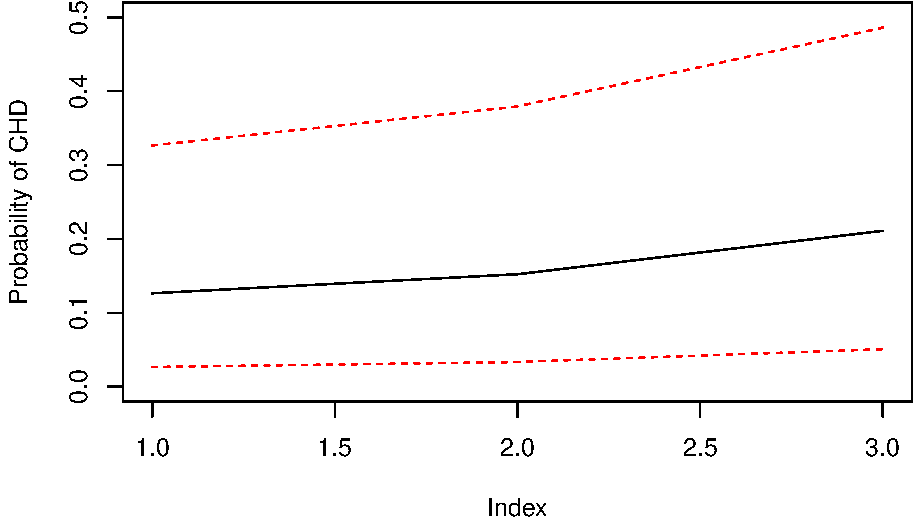
\includegraphics{framingham_files/figure-latex/unnamed-chunk-9-1.pdf}

\subsubsection{IPTW}\label{iptw-1}

\begin{Shaded}
\begin{Highlighting}[]
\NormalTok{### Create pairwise binary variables for each bin}
\NormalTok{fhs_binned}\OperatorTok{$}\NormalTok{cigsPerDay_bin_}\DecValTok{1}\NormalTok{ <-}\StringTok{ }\KeywordTok{ifelse}\NormalTok{(fhs_binned}\OperatorTok{$}\NormalTok{cigsPerDay }\OperatorTok{==}\StringTok{ "[0, 0.9)"}\NormalTok{,}\DecValTok{1}\NormalTok{,}\DecValTok{0}\NormalTok{)}
\NormalTok{fhs_binned}\OperatorTok{$}\NormalTok{cigsPerDay_bin_}\DecValTok{2}\NormalTok{ <-}\StringTok{ }\KeywordTok{ifelse}\NormalTok{(fhs_binned}\OperatorTok{$}\NormalTok{cigsPerDay }\OperatorTok{==}\StringTok{ "[0.9, 20)"}\NormalTok{,}\DecValTok{1}\NormalTok{,}\DecValTok{0}\NormalTok{)}
\NormalTok{fhs_binned}\OperatorTok{$}\NormalTok{cigsPerDay_bin_}\DecValTok{3}\NormalTok{ <-}\StringTok{ }\KeywordTok{ifelse}\NormalTok{(fhs_binned}\OperatorTok{$}\NormalTok{cigsPerDay }\OperatorTok{==}\StringTok{ "[20, 70]"}\NormalTok{,}\DecValTok{1}\NormalTok{,}\DecValTok{0}\NormalTok{)}

\NormalTok{### BIN 2}
\NormalTok{glm_fit_iptw_bin_}\DecValTok{1}\NormalTok{ <-}\StringTok{ }\KeywordTok{glm}\NormalTok{( cigsPerDay_bin_}\DecValTok{1} \OperatorTok{~}\StringTok{   }\NormalTok{education }\OperatorTok{+}\StringTok{ }\NormalTok{age }\OperatorTok{+}\StringTok{ }\NormalTok{diabetes }\OperatorTok{+}\StringTok{ }\NormalTok{bmi , }\DataTypeTok{data =}\NormalTok{ fhs_binned, }\DataTypeTok{family =} \StringTok{"binomial"}\NormalTok{)}
\NormalTok{prob.1W <-}\StringTok{ }\KeywordTok{predict}\NormalTok{(glm_fit_iptw_bin_}\DecValTok{1}\NormalTok{, }\DataTypeTok{type=} \StringTok{"response"}\NormalTok{)}
\NormalTok{wt_}\DecValTok{1}\NormalTok{<-}\StringTok{ }\DecValTok{1}\OperatorTok{/}\NormalTok{prob.1W}
\KeywordTok{summary}\NormalTok{(wt_}\DecValTok{1}\NormalTok{)}
\end{Highlighting}
\end{Shaded}

\begin{verbatim}
##    Min. 1st Qu.  Median    Mean 3rd Qu.    Max. 
##   1.174   1.624   1.973   2.094   2.470   3.962
\end{verbatim}

\begin{Shaded}
\begin{Highlighting}[]
\NormalTok{IPTW_bin_}\DecValTok{1}\NormalTok{<-}\StringTok{ }\KeywordTok{mean}\NormalTok{( wt_}\DecValTok{1}\OperatorTok{*}\KeywordTok{as.numeric}\NormalTok{(fhs_binned}\OperatorTok{$}\NormalTok{cigsPerDay_bin_}\DecValTok{1}\OperatorTok{==}\DecValTok{1}\NormalTok{)}\OperatorTok{*}\KeywordTok{as.numeric}\NormalTok{(fhs_binned}\OperatorTok{$}\NormalTok{CHD}\OperatorTok{==}\DecValTok{1}\NormalTok{))}

\NormalTok{### BIN 2}
\NormalTok{glm_fit_iptw_bin_}\DecValTok{2}\NormalTok{ <-}\StringTok{ }\KeywordTok{glm}\NormalTok{( cigsPerDay_bin_}\DecValTok{2} \OperatorTok{~}\StringTok{   }\NormalTok{education }\OperatorTok{+}\StringTok{ }\NormalTok{age }\OperatorTok{+}\StringTok{ }\NormalTok{diabetes }\OperatorTok{+}\StringTok{ }\NormalTok{bmi , }\DataTypeTok{data =}\NormalTok{ fhs_binned, }\DataTypeTok{family =} \StringTok{"binomial"}\NormalTok{)}
\NormalTok{prob.1W <-}\StringTok{ }\KeywordTok{predict}\NormalTok{(glm_fit_iptw_bin_}\DecValTok{2}\NormalTok{, }\DataTypeTok{type=} \StringTok{"response"}\NormalTok{)}
\NormalTok{wt_}\DecValTok{2}\NormalTok{<-}\StringTok{ }\DecValTok{1}\OperatorTok{/}\NormalTok{prob.1W}
\KeywordTok{summary}\NormalTok{(wt_}\DecValTok{2}\NormalTok{)}
\end{Highlighting}
\end{Shaded}

\begin{verbatim}
##    Min. 1st Qu.  Median    Mean 3rd Qu.    Max. 
##   2.476   3.895   5.272   5.445   6.456  12.287
\end{verbatim}

\begin{Shaded}
\begin{Highlighting}[]
\NormalTok{IPTW_bin_}\DecValTok{2}\NormalTok{<-}\StringTok{ }\KeywordTok{mean}\NormalTok{( wt_}\DecValTok{2}\OperatorTok{*}\KeywordTok{as.numeric}\NormalTok{(fhs_binned}\OperatorTok{$}\NormalTok{cigsPerDay_bin_}\DecValTok{2}\OperatorTok{==}\DecValTok{1}\NormalTok{)}\OperatorTok{*}\KeywordTok{as.numeric}\NormalTok{(fhs_binned}\OperatorTok{$}\NormalTok{CHD}\OperatorTok{==}\DecValTok{1}\NormalTok{))}

\NormalTok{### BIN 3}
\NormalTok{glm_fit_iptw_bin_}\DecValTok{3}\NormalTok{ <-}\StringTok{ }\KeywordTok{glm}\NormalTok{( cigsPerDay_bin_}\DecValTok{3} \OperatorTok{~}\StringTok{   }\NormalTok{education }\OperatorTok{+}\StringTok{ }\NormalTok{age }\OperatorTok{+}\StringTok{ }\NormalTok{diabetes }\OperatorTok{+}\StringTok{ }\NormalTok{bmi , }\DataTypeTok{data =}\NormalTok{ fhs_binned, }\DataTypeTok{family =} \StringTok{"binomial"}\NormalTok{)}
\NormalTok{prob.1W <-}\StringTok{ }\KeywordTok{predict}\NormalTok{(glm_fit_iptw_bin_}\DecValTok{3}\NormalTok{, }\DataTypeTok{type=} \StringTok{"response"}\NormalTok{)}
\NormalTok{wt_}\DecValTok{3}\NormalTok{<-}\StringTok{ }\DecValTok{1}\OperatorTok{/}\NormalTok{prob.1W}
\KeywordTok{summary}\NormalTok{(wt_}\DecValTok{3}\NormalTok{)}
\end{Highlighting}
\end{Shaded}

\begin{verbatim}
##    Min. 1st Qu.  Median    Mean 3rd Qu.    Max. 
##   2.340   2.818   3.327   3.927   4.520  13.164
\end{verbatim}

\begin{Shaded}
\begin{Highlighting}[]
\NormalTok{IPTW_bin_}\DecValTok{3}\NormalTok{<-}\StringTok{ }\KeywordTok{mean}\NormalTok{( wt_}\DecValTok{3}\OperatorTok{*}\KeywordTok{as.numeric}\NormalTok{(fhs_binned}\OperatorTok{$}\NormalTok{cigsPerDay_bin_}\DecValTok{3}\OperatorTok{==}\DecValTok{1}\NormalTok{)}\OperatorTok{*}\KeywordTok{as.numeric}\NormalTok{(fhs_binned}\OperatorTok{$}\NormalTok{CHD}\OperatorTok{==}\DecValTok{1}\NormalTok{))}

\KeywordTok{plot}\NormalTok{(}\KeywordTok{c}\NormalTok{(IPTW_bin_}\DecValTok{1}\NormalTok{,IPTW_bin_}\DecValTok{2}\NormalTok{,IPTW_bin_}\DecValTok{3}\NormalTok{),}\DataTypeTok{type=}\StringTok{'l'}\NormalTok{,}\DataTypeTok{col=}\StringTok{'blue'}\NormalTok{)}
\end{Highlighting}
\end{Shaded}

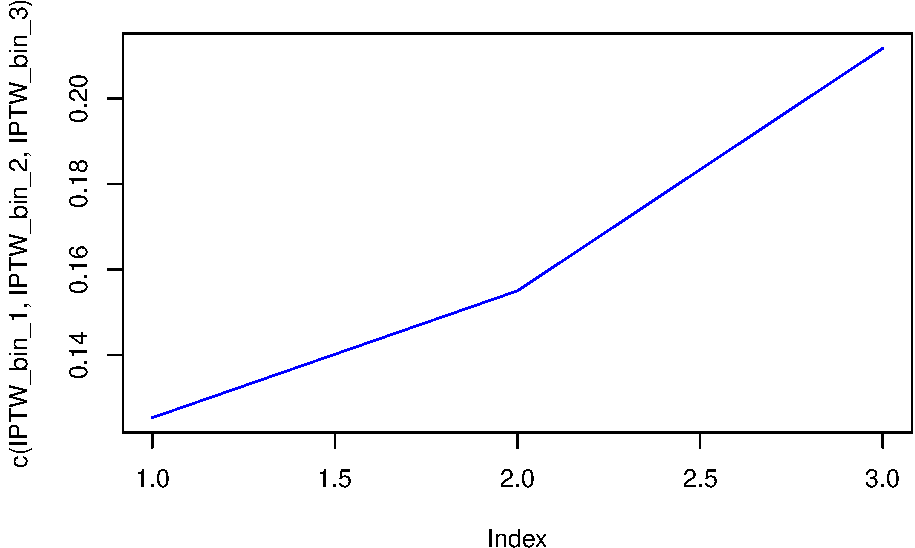
\includegraphics{framingham_files/figure-latex/unnamed-chunk-10-1.pdf}

\subsubsection{Superlearner/TMLE}\label{superlearnertmle}

BIN 3

\begin{Shaded}
\begin{Highlighting}[]
\KeywordTok{library}\NormalTok{(}\StringTok{'SuperLearner'}\NormalTok{)}
\end{Highlighting}
\end{Shaded}

\begin{verbatim}
## Loading required package: nnls
\end{verbatim}

\begin{verbatim}
## Super Learner
\end{verbatim}

\begin{verbatim}
## Version: 2.0-24
\end{verbatim}

\begin{verbatim}
## Package created on 2018-08-10
\end{verbatim}

\begin{Shaded}
\begin{Highlighting}[]
\NormalTok{SL.library<-}\StringTok{ }\KeywordTok{c}\NormalTok{(}\StringTok{"SL.glmnet"}\NormalTok{)}


\NormalTok{### Bin1 TMLE}

\NormalTok{X_minus_bin_}\DecValTok{1}\NormalTok{<-}\StringTok{ }\KeywordTok{subset}\NormalTok{(fhs_binned, }\DataTypeTok{select=} \KeywordTok{c}\NormalTok{(}\StringTok{"cigsPerDay_bin_1"}\NormalTok{, }\StringTok{"education"}\NormalTok{, }\StringTok{"age"}\NormalTok{,}\StringTok{"diabetes"}\NormalTok{,}\StringTok{"bmi"}\NormalTok{) )}
\NormalTok{X_minus_bin_1_all_bin_}\DecValTok{1}\NormalTok{ <-}\StringTok{ }\NormalTok{X_minus_bin_}\DecValTok{1}
\NormalTok{X_minus_bin_1_all_bin_}\DecValTok{1}\OperatorTok{$}\NormalTok{cigsPerDay_bin_}\DecValTok{1}\NormalTok{ <-}\StringTok{ }\DecValTok{1}
\NormalTok{SL.outcome<-}\StringTok{ }\KeywordTok{SuperLearner}\NormalTok{(}\DataTypeTok{Y=}\KeywordTok{as.numeric}\NormalTok{(fhs_binned}\OperatorTok{$}\NormalTok{CHD}\OperatorTok{==}\DecValTok{1}\NormalTok{), }\DataTypeTok{X=}\NormalTok{X_minus_bin_}\DecValTok{1}\NormalTok{, }\DataTypeTok{SL.library=}\NormalTok{SL.library, }\DataTypeTok{family=}\StringTok{"binomial"}\NormalTok{)}
\end{Highlighting}
\end{Shaded}

\begin{verbatim}
## Loading required package: glmnet
\end{verbatim}

\begin{verbatim}
## Loading required package: Matrix
\end{verbatim}

\begin{verbatim}
## Loading required package: foreach
\end{verbatim}

\begin{verbatim}
## Loaded glmnet 2.0-16
\end{verbatim}

\begin{Shaded}
\begin{Highlighting}[]
\NormalTok{expY.givenA1 <-}\StringTok{  }\KeywordTok{predict}\NormalTok{(SL.outcome, }\DataTypeTok{newdata=}\NormalTok{X_minus_bin_1_all_bin_}\DecValTok{1}\NormalTok{)}\OperatorTok{$}\NormalTok{pred}
\NormalTok{SL.exposure<-}\StringTok{ }\KeywordTok{SuperLearner}\NormalTok{(}\DataTypeTok{Y=}\KeywordTok{as.numeric}\NormalTok{(fhs_binned}\OperatorTok{$}\NormalTok{cigsPerDay_bin_}\DecValTok{1}\OperatorTok{==}\DecValTok{1}\NormalTok{), }\DataTypeTok{X=}\KeywordTok{subset}\NormalTok{(X_minus_bin_}\DecValTok{1}\NormalTok{, }\DataTypeTok{select=} \OperatorTok{-}\KeywordTok{c}\NormalTok{(cigsPerDay_bin_}\DecValTok{1}\NormalTok{)),}\DataTypeTok{SL.library=}\NormalTok{SL.library, }\DataTypeTok{family=}\StringTok{"binomial"}\NormalTok{)}
\NormalTok{probA1.givenW<-}\StringTok{ }\NormalTok{SL.exposure}\OperatorTok{$}\NormalTok{SL.predict}
\NormalTok{H.AW<-}\StringTok{ }\KeywordTok{as.numeric}\NormalTok{(fhs_binned}\OperatorTok{$}\NormalTok{cigsPerDay_bin_}\DecValTok{1}\OperatorTok{==}\DecValTok{1}\NormalTok{)}\OperatorTok{/}\NormalTok{probA1.givenW}
\NormalTok{logitUpdate<-}\StringTok{ }\KeywordTok{glm}\NormalTok{(fhs_binned}\OperatorTok{$}\NormalTok{CHD }\OperatorTok{~}\StringTok{ }\OperatorTok{-}\DecValTok{1} \OperatorTok{+}\KeywordTok{offset}\NormalTok{(}\KeywordTok{qlogis}\NormalTok{(expY.givenA1)) }\OperatorTok{+}\StringTok{ }\NormalTok{H.AW, }\DataTypeTok{family=}\StringTok{'binomial'}\NormalTok{)}
\NormalTok{epsilon<-}\StringTok{ }\NormalTok{logitUpdate}\OperatorTok{$}\NormalTok{coef}
\NormalTok{expY.givenAW.star<-}\StringTok{ }\KeywordTok{plogis}\NormalTok{(}\KeywordTok{qlogis}\NormalTok{(expY.givenA1)}\OperatorTok{+}\StringTok{ }\NormalTok{epsilon}\OperatorTok{*}\NormalTok{H.AW)}
\NormalTok{PsiHat.TMLE_bin_}\DecValTok{1}\NormalTok{<-}\StringTok{ }\KeywordTok{mean}\NormalTok{(expY.givenAW.star)}\CommentTok{#- expY.given0W.star)}


\NormalTok{X_minus_bin_}\DecValTok{2}\NormalTok{<-}\StringTok{ }\KeywordTok{subset}\NormalTok{(fhs_binned, }\DataTypeTok{select=} \KeywordTok{c}\NormalTok{(}\StringTok{"cigsPerDay_bin_2"}\NormalTok{, }\StringTok{"education"}\NormalTok{, }\StringTok{"age"}\NormalTok{,}\StringTok{"diabetes"}\NormalTok{,}\StringTok{"bmi"}\NormalTok{) )}
\NormalTok{X_minus_bin_2_all_bin_}\DecValTok{2}\NormalTok{ <-}\StringTok{ }\NormalTok{X_minus_bin_}\DecValTok{2}
\NormalTok{X_minus_bin_2_all_bin_}\DecValTok{2}\OperatorTok{$}\NormalTok{cigsPerDay_bin_}\DecValTok{2}\NormalTok{ <-}\StringTok{ }\DecValTok{1}
\NormalTok{SL.outcome<-}\StringTok{ }\KeywordTok{SuperLearner}\NormalTok{(}\DataTypeTok{Y=}\KeywordTok{as.numeric}\NormalTok{(fhs_binned}\OperatorTok{$}\NormalTok{CHD}\OperatorTok{==}\DecValTok{1}\NormalTok{), }\DataTypeTok{X=}\NormalTok{X_minus_bin_}\DecValTok{2}\NormalTok{, }\DataTypeTok{SL.library=}\NormalTok{SL.library, }\DataTypeTok{family=}\StringTok{"binomial"}\NormalTok{)}
\NormalTok{expY.givenA1 <-}\StringTok{  }\KeywordTok{predict}\NormalTok{(SL.outcome, }\DataTypeTok{newdata=}\NormalTok{X_minus_bin_2_all_bin_}\DecValTok{2}\NormalTok{)}\OperatorTok{$}\NormalTok{pred}
\NormalTok{SL.exposure<-}\StringTok{ }\KeywordTok{SuperLearner}\NormalTok{(}\DataTypeTok{Y=}\KeywordTok{as.numeric}\NormalTok{(fhs_binned}\OperatorTok{$}\NormalTok{cigsPerDay_bin_}\DecValTok{2}\OperatorTok{==}\DecValTok{1}\NormalTok{), }\DataTypeTok{X=}\KeywordTok{subset}\NormalTok{(X_minus_bin_}\DecValTok{2}\NormalTok{, }\DataTypeTok{select=} \OperatorTok{-}\KeywordTok{c}\NormalTok{(cigsPerDay_bin_}\DecValTok{2}\NormalTok{)),}\DataTypeTok{SL.library=}\NormalTok{SL.library, }\DataTypeTok{family=}\StringTok{"binomial"}\NormalTok{)}
\NormalTok{probA1.givenW<-}\StringTok{ }\NormalTok{SL.exposure}\OperatorTok{$}\NormalTok{SL.predict}
\NormalTok{H.AW<-}\StringTok{ }\KeywordTok{as.numeric}\NormalTok{(fhs_binned}\OperatorTok{$}\NormalTok{cigsPerDay_bin_}\DecValTok{2}\OperatorTok{==}\DecValTok{1}\NormalTok{)}\OperatorTok{/}\NormalTok{probA1.givenW}
\NormalTok{logitUpdate<-}\StringTok{ }\KeywordTok{glm}\NormalTok{(fhs_binned}\OperatorTok{$}\NormalTok{CHD }\OperatorTok{~}\StringTok{ }\OperatorTok{-}\DecValTok{1} \OperatorTok{+}\KeywordTok{offset}\NormalTok{(}\KeywordTok{qlogis}\NormalTok{(expY.givenA1)) }\OperatorTok{+}\StringTok{ }\NormalTok{H.AW, }\DataTypeTok{family=}\StringTok{'binomial'}\NormalTok{)}
\NormalTok{epsilon<-}\StringTok{ }\NormalTok{logitUpdate}\OperatorTok{$}\NormalTok{coef}
\NormalTok{expY.givenAW.star<-}\StringTok{ }\KeywordTok{plogis}\NormalTok{(}\KeywordTok{qlogis}\NormalTok{(expY.givenA1)}\OperatorTok{+}\StringTok{ }\NormalTok{epsilon}\OperatorTok{*}\NormalTok{H.AW)}
\NormalTok{PsiHat.TMLE_bin_}\DecValTok{2}\NormalTok{<-}\StringTok{ }\KeywordTok{mean}\NormalTok{(expY.givenAW.star)}\CommentTok{#- expY.given0W.star)}
\NormalTok{#### BIN 3 TMLE }

\NormalTok{X_minus_bin_}\DecValTok{3}\NormalTok{<-}\StringTok{ }\KeywordTok{subset}\NormalTok{(fhs_binned, }\DataTypeTok{select=} \KeywordTok{c}\NormalTok{(}\StringTok{"cigsPerDay_bin_3"}\NormalTok{, }\StringTok{"education"}\NormalTok{, }\StringTok{"age"}\NormalTok{,}\StringTok{"diabetes"}\NormalTok{,}\StringTok{"bmi"}\NormalTok{) )}
\NormalTok{X_minus_bin_3_all_bin_}\DecValTok{3}\NormalTok{ <-}\StringTok{ }\NormalTok{X_minus_bin_}\DecValTok{3}
\NormalTok{X_minus_bin_3_all_bin_}\DecValTok{3}\OperatorTok{$}\NormalTok{cigsPerDay_bin_}\DecValTok{3}\NormalTok{ <-}\StringTok{ }\DecValTok{1}
\NormalTok{SL.outcome<-}\StringTok{ }\KeywordTok{SuperLearner}\NormalTok{(}\DataTypeTok{Y=}\KeywordTok{as.numeric}\NormalTok{(fhs_binned}\OperatorTok{$}\NormalTok{CHD}\OperatorTok{==}\DecValTok{1}\NormalTok{), }\DataTypeTok{X=}\NormalTok{X_minus_bin_}\DecValTok{3}\NormalTok{, }\DataTypeTok{SL.library=}\NormalTok{SL.library, }\DataTypeTok{family=}\StringTok{"binomial"}\NormalTok{)}
\NormalTok{expY.givenA1 <-}\StringTok{  }\KeywordTok{predict}\NormalTok{(SL.outcome, }\DataTypeTok{newdata=}\NormalTok{X_minus_bin_3_all_bin_}\DecValTok{3}\NormalTok{)}\OperatorTok{$}\NormalTok{pred}
\NormalTok{SL.exposure<-}\StringTok{ }\KeywordTok{SuperLearner}\NormalTok{(}\DataTypeTok{Y=}\KeywordTok{as.numeric}\NormalTok{(fhs_binned}\OperatorTok{$}\NormalTok{cigsPerDay_bin_}\DecValTok{3}\OperatorTok{==}\DecValTok{1}\NormalTok{), }\DataTypeTok{X=}\KeywordTok{subset}\NormalTok{(X_minus_bin_}\DecValTok{3}\NormalTok{, }\DataTypeTok{select=} \OperatorTok{-}\KeywordTok{c}\NormalTok{(cigsPerDay_bin_}\DecValTok{3}\NormalTok{)),}\DataTypeTok{SL.library=}\NormalTok{SL.library, }\DataTypeTok{family=}\StringTok{"binomial"}\NormalTok{)}
\NormalTok{probA1.givenW<-}\StringTok{ }\NormalTok{SL.exposure}\OperatorTok{$}\NormalTok{SL.predict}
\NormalTok{H.AW<-}\StringTok{ }\KeywordTok{as.numeric}\NormalTok{(fhs_binned}\OperatorTok{$}\NormalTok{cigsPerDay_bin_}\DecValTok{3}\OperatorTok{==}\DecValTok{1}\NormalTok{)}\OperatorTok{/}\NormalTok{probA1.givenW}
\NormalTok{logitUpdate<-}\StringTok{ }\KeywordTok{glm}\NormalTok{(fhs_binned}\OperatorTok{$}\NormalTok{CHD }\OperatorTok{~}\StringTok{ }\OperatorTok{-}\DecValTok{1} \OperatorTok{+}\KeywordTok{offset}\NormalTok{(}\KeywordTok{qlogis}\NormalTok{(expY.givenA1)) }\OperatorTok{+}\StringTok{ }\NormalTok{H.AW, }\DataTypeTok{family=}\StringTok{'binomial'}\NormalTok{)}
\NormalTok{epsilon<-}\StringTok{ }\NormalTok{logitUpdate}\OperatorTok{$}\NormalTok{coef}
\NormalTok{expY.givenAW.star<-}\StringTok{ }\KeywordTok{plogis}\NormalTok{(}\KeywordTok{qlogis}\NormalTok{(expY.givenA1)}\OperatorTok{+}\StringTok{ }\NormalTok{epsilon}\OperatorTok{*}\NormalTok{H.AW)}
\NormalTok{PsiHat.TMLE_bin_}\DecValTok{3}\NormalTok{ <-}\StringTok{ }\KeywordTok{mean}\NormalTok{(expY.givenAW.star)}\CommentTok{#- expY.given0W.star)}
\end{Highlighting}
\end{Shaded}

\begin{Shaded}
\begin{Highlighting}[]
\KeywordTok{plot}\NormalTok{(}\KeywordTok{c}\NormalTok{(PsiHat.TMLE_bin_}\DecValTok{1}\NormalTok{,PsiHat.TMLE_bin_}\DecValTok{2}\NormalTok{,PsiHat.TMLE_bin_}\DecValTok{3}\NormalTok{),}\DataTypeTok{type=}\StringTok{'l'}\NormalTok{,}\DataTypeTok{ylab=}\StringTok{"TMLE"}\NormalTok{)}
\end{Highlighting}
\end{Shaded}

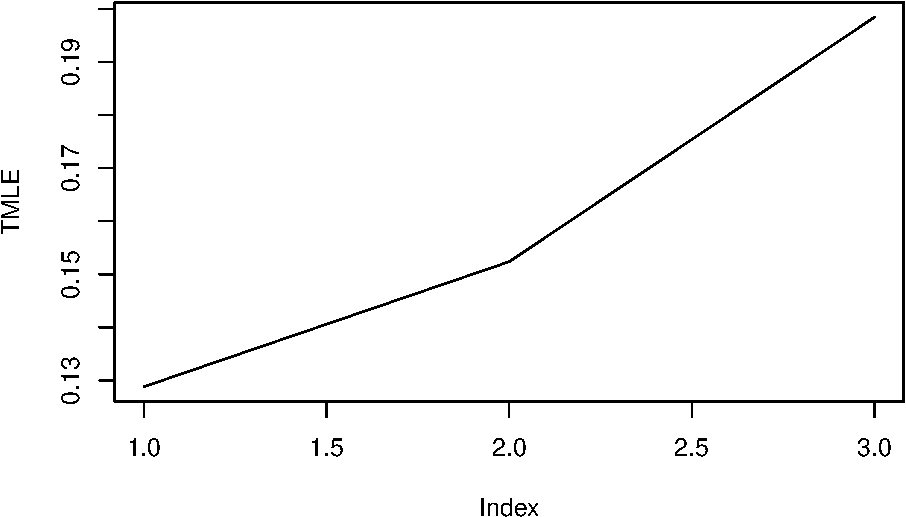
\includegraphics{framingham_files/figure-latex/unnamed-chunk-12-1.pdf}

\subsection{Step 7. Result
Interpretation}\label{step-7.-result-interpretation}

What is the statistical interpretation of your analyses? Discuss
differences (or lack thereof) in the estimates provided by the different
estimators. What is the causal interpretation of your results and how
plausible is it? What are key limitations of your analysis? How might
these results (if at all) inform policy, understanding, and/or the
design of future studies?


\end{document}
